


\tikzset{every picture/.style={line width=0.75pt}} %set default line width to 0.75pt        

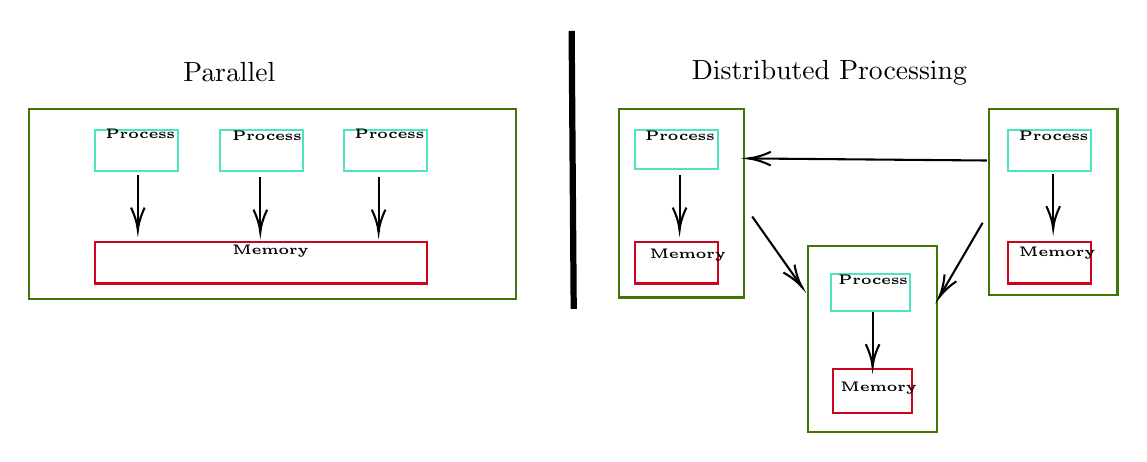
\begin{tikzpicture}[x=0.75pt,y=0.75pt,yscale=-1,xscale=1]
	%uncomment if require: \path (0,415); %set diagram left start at 0, and has height of 415
	
	%Shape: Rectangle [id:dp8655887794683795] 
	\draw  [color={rgb, 255:red, 65; green, 117; blue, 5 }  ,draw opacity=1 ] (18,111) -- (252.58,111) -- (252.58,202.25) -- (18,202.25) -- cycle ;
	%Shape: Rectangle [id:dp8907085252035312] 
	\draw  [color={rgb, 255:red, 65; green, 117; blue, 5 }  ,draw opacity=1 ] (302.58,111) -- (362.58,111) -- (362.58,201.75) -- (302.58,201.75) -- cycle ;
	%Shape: Rectangle [id:dp531973268669913] 
	\draw  [color={rgb, 255:red, 80; green, 227; blue, 194 }  ,draw opacity=1 ] (50,121) -- (90,121) -- (90,141) -- (50,141) -- cycle ;
	%Shape: Rectangle [id:dp32192612836678103] 
	\draw  [color={rgb, 255:red, 80; green, 227; blue, 194 }  ,draw opacity=1 ] (110,121) -- (150,121) -- (150,141) -- (110,141) -- cycle ;
	%Shape: Rectangle [id:dp972266177760866] 
	\draw  [color={rgb, 255:red, 80; green, 227; blue, 194 }  ,draw opacity=1 ] (170,121) -- (210,121) -- (210,141) -- (170,141) -- cycle ;
	%Rounded Rect [id:dp763489432971651] 
	\draw  [color={rgb, 255:red, 208; green, 2; blue, 27 }  ,draw opacity=1 ] 
	 (50,175) -- (210,175) -- (210,195) -- (50,195) -- cycle ;-- cycle ;
	%Shape: Rectangle [id:dp46420165615263753] 
	\draw  [color={rgb, 255:red, 65; green, 117; blue, 5 }  ,draw opacity=1 ] (480.58,111) -- (542.58,111) -- (542.58,200.75) -- (480.58,200.75) -- cycle ;
	%Shape: Rectangle [id:dp27479252331465176] 
	\draw  [color={rgb, 255:red, 65; green, 117; blue, 5 }  ,draw opacity=1 ] (393.58,177) -- (455.58,177) -- (455.58,266.75) -- (393.58,266.75) -- cycle ;
	%Straight Lines [id:da369260676335904] 
	\draw [line width=2.25]    (279.58,73.25) -- (280.58,207.25) ;
	%Shape: Rectangle [id:dp7935185593682178] 
	\draw  [color={rgb, 255:red, 80; green, 227; blue, 194 }  ,draw opacity=1 ] (310,121) -- (350,121) -- (350,140) -- (310,140) -- cycle ;
	%Shape: Rectangle [id:dp34622696632931327]   % memory box 2
	\draw  [color={rgb, 255:red, 208; green, 2; blue, 27 }  ,draw opacity=1 ] (310,175) -- (350,175) -- (350,195) -- (310,195) -- cycle ;
	%Shape: Rectangle [id:dp00038374666294560544] 
	\draw  [color={rgb, 255:red, 80; green, 227; blue, 194 }  ,draw opacity=1 ] (404.58,190.25) -- (442.58,190.25) -- (442.58,208.25) -- (404.58,208.25) -- cycle ;
	%Shape: Rectangle [id:dp3209647982053657] 
	\draw  [color={rgb, 255:red, 80; green, 227; blue, 194 }  ,draw opacity=1 ] (490,121) -- (530,121) -- (530,141) -- (490,141) -- cycle ;
	%Shape: Rectangle [id:dp8025652037528683]  %memory box 4
	\draw  [color={rgb, 255:red, 208; green, 2; blue, 27 }  ,draw opacity=1 ] (405.58,236.25) -- (443.58,236.25) -- (443.58,257.25) -- (405.58,257.25) -- cycle ;
	%Shape: Rectangle [id:dp2266373468363876]  % memory box 3
	\draw  [color={rgb, 255:red, 208; green, 2; blue, 27 }  ,draw opacity=1 ] (490,175) -- (530,175) -- (530,195) -- (490,195) -- cycle ;
	%Straight Lines [id:da5029820921379233] 
	\draw    (331.58,142.75) -- (331.58,167.38) ;
	\draw [shift={(331.58,169.38)}, rotate = 270] [color={rgb, 255:red, 0; green, 0; blue, 0 }  ][line width=0.75]    (10.93,-3.29) .. controls (6.95,-1.4) and (3.31,-0.3) .. (0,0) .. controls (3.31,0.3) and (6.95,1.4) .. (10.93,3.29)   ;
	%Straight Lines [id:da7730658410797611] 
	\draw    (424.58,208.56) -- (424.58,233.19) ;
	\draw [shift={(424.58,235.19)}, rotate = 270] [color={rgb, 255:red, 0; green, 0; blue, 0 }  ][line width=0.75]    (10.93,-3.29) .. controls (6.95,-1.4) and (3.31,-0.3) .. (0,0) .. controls (3.31,0.3) and (6.95,1.4) .. (10.93,3.29)   ;
	%Straight Lines [id:da9994794173682501] 
	\draw    (511.58,142.06) -- (511.58,166.69) ;
	\draw [shift={(511.58,168.69)}, rotate = 270] [color={rgb, 255:red, 0; green, 0; blue, 0 }  ][line width=0.75]    (10.93,-3.29) .. controls (6.95,-1.4) and (3.31,-0.3) .. (0,0) .. controls (3.31,0.3) and (6.95,1.4) .. (10.93,3.29)   ;
	%Straight Lines [id:da9705771813095805] 
	\draw    (186.58,143.75) -- (186.58,168.38) ;
	\draw [shift={(186.58,170.38)}, rotate = 270] [color={rgb, 255:red, 0; green, 0; blue, 0 }  ][line width=0.75]    (10.93,-3.29) .. controls (6.95,-1.4) and (3.31,-0.3) .. (0,0) .. controls (3.31,0.3) and (6.95,1.4) .. (10.93,3.29)   ;
	%Straight Lines [id:da5879748150918536] 
	\draw    (129.58,143.75) -- (129.58,168.38) ;
	\draw [shift={(129.58,170.38)}, rotate = 270] [color={rgb, 255:red, 0; green, 0; blue, 0 }  ][line width=0.75]    (10.93,-3.29) .. controls (6.95,-1.4) and (3.31,-0.3) .. (0,0) .. controls (3.31,0.3) and (6.95,1.4) .. (10.93,3.29)   ;
	%Straight Lines [id:da6653546271183027] 
	\draw    (70.58,142.75) -- (70.58,167.38) ;
	\draw [shift={(70.58,169.38)}, rotate = 270] [color={rgb, 255:red, 0; green, 0; blue, 0 }  ][line width=0.75]    (10.93,-3.29) .. controls (6.95,-1.4) and (3.31,-0.3) .. (0,0) .. controls (3.31,0.3) and (6.95,1.4) .. (10.93,3.29)   ;
	%Straight Lines [id:da9386491963364736] 
	\draw    (366.58,162.75) -- (389.43,195.12) ;
	\draw [shift={(390.58,196.75)}, rotate = 234.78] [color={rgb, 255:red, 0; green, 0; blue, 0 }  ][line width=0.75]    (10.93,-3.29) .. controls (6.95,-1.4) and (3.31,-0.3) .. (0,0) .. controls (3.31,0.3) and (6.95,1.4) .. (10.93,3.29)   ;
	%Straight Lines [id:da5731244822727878] 
	\draw    (477.58,165.75) -- (457.59,200.02) ;
	\draw [shift={(456.58,201.75)}, rotate = 300.26] [color={rgb, 255:red, 0; green, 0; blue, 0 }  ][line width=0.75]    (10.93,-3.29) .. controls (6.95,-1.4) and (3.31,-0.3) .. (0,0) .. controls (3.31,0.3) and (6.95,1.4) .. (10.93,3.29)   ;
	%Straight Lines [id:da06900608847320588] 
	\draw    (479.58,135.75) -- (366.58,134.77) ;
	\draw [shift={(364.58,134.75)}, rotate = 360.5] [color={rgb, 255:red, 0; green, 0; blue, 0 }  ][line width=0.75]    (10.93,-3.29) .. controls (6.95,-1.4) and (3.31,-0.3) .. (0,0) .. controls (3.31,0.3) and (6.95,1.4) .. (10.93,3.29)   ;
	
	% Text Node
	\draw (91,87) node [anchor=north west][inner sep=0.75pt]   [align=left] {Parallel};
	% Text Node
	\draw (336,86) node [anchor=north west][inner sep=0.75pt]   [align=left] {Distributed Processing};
	% Text Node
	\draw (114.42,175) node [anchor=north west][inner sep=0.75pt]  [font=\tiny,xslant=-0.07] [align=left] {\textbf{Memory}};
	% Text Node
	\draw (315.42,177) node [anchor=north west][inner sep=0.75pt]  [font=\tiny,xslant=-0.07] [align=left] {\textbf{Memory}};
	% Text Node
	\draw (53.58,119) node [anchor=north west][inner sep=0.75pt]   [align=left] {{\tiny \textbf{Process}}};
	% Text Node
	\draw (114.58,120) node [anchor=north west][inner sep=0.75pt]   [align=left] {{\tiny \textbf{Process}}};
	% Text Node
	\draw (173.58,119.25) node [anchor=north west][inner sep=0.75pt]   [align=left] {{\tiny \textbf{Process}}};
	% Text Node
	\draw (313.58,120.25) node [anchor=north west][inner sep=0.75pt]   [align=left] {{\tiny \textbf{Process}}};
	% Text Node
	\draw (406.58,189.25) node [anchor=north west][inner sep=0.75pt]   [align=left] {{\tiny \textbf{Process}}};
	% Text Node
	\draw (493.58,120.25) node [anchor=north west][inner sep=0.75pt]   [align=left] {{\tiny \textbf{Process}}};
	% Text Node
	\draw (407.42,241) node [anchor=north west][inner sep=0.75pt]  [font=\tiny,xslant=-0.07] [align=left] {\textbf{Memory}};
	% Text Node
	\draw (493.42,176) node [anchor=north west][inner sep=0.75pt]  [font=\tiny,xslant=-0.07] [align=left] {\textbf{Memory}};
	
	
\end{tikzpicture}
